\chapter{Reproducibility and Training Dynamics}
\label{app:reproducibility}

This appendix provides supplementary material to ensure the full reproducibility of the experiments discussed in Chapter~\ref{cha:results}.
It includes the complete configuration files used for training the generative models, alongside detailed plots illustrating the training dynamics, the statistical matching achieved, and the qualitative evolution of the generated radargrams across epochs.

\section{Complete Configuration Files}
The following listings report the exact YAML configuration files utilized for the final training runs. 

\subsection{CycleGAN Configuration}
\begin{lstlisting}[basicstyle=\ttfamily\footnotesize, frame=single, breaklines=true]
DEVICE: "cuda"
GENERATOR_LEARNING_RATE: 2e-4
DISCRIMINATOR_LEARNING_RATE: 1e-4
BATCH_SIZE: 1
NUM_WORKERS: 2
PATCH_SIZE: 128
PATCH_OVERLAP: 0
CHANNELS_IMG: 1
L1_LAMBDA: 100
NUM_EPOCHS: 40
LABEL_SMOOTHING: 0.0
NORMALIZATION_TYPE: "range_minus_one_to_one"
MODEL_NAME: cyclegan
DISCRIMINATOR_RECEPTIVE_FIELD: "34x34"
LAMBDA_CYCLE: 10.0
LAMBDA_IDENTITY: 0.5
USE_AMP: true
\end{lstlisting}

\subsection{Pix2Pix Configuration}
\begin{lstlisting}[basicstyle=\ttfamily\footnotesize, frame=single, breaklines=true]
DEVICE: "cuda"
GENERATOR_LEARNING_RATE: 2e-5
DISCRIMINATOR_LEARNING_RATE: 1e-5
BATCH_SIZE: 1
NUM_WORKERS: 2
PATCH_SIZE: 128
PATCH_OVERLAP: 0
CHANNELS_IMG: 1
L1_LAMBDA: 100
NUM_EPOCHS: 60
LABEL_SMOOTHING: 0.0
NORMALIZATION_TYPE: "range_minus_one_to_one"
MODEL_NAME: pix2pix
DISCRIMINATOR_RECEPTIVE_FIELD: "34x34"
USE_AMP: false
\end{lstlisting}

\clearpage

\section{Statistical Match: Distributions and Rangelines}
To further validate the physical realism of the synthesized data, the following figures compare the statistical properties of the generated radargrams against the real SHARAD observations.
Figure~\ref{fig:app_distributions} evaluates the overall pixel intensity distributions for both models, while Figure~\ref{fig:app_rangelines} compares the average vertical rangelines, illustrating how well each architecture captures the depth-dependent signal attenuation at the end of the training process.

% --- FIGURA 1: DISTRIBUTIONS ---
\begin{figure}[htbp]
    \centering
    % CycleGAN Distribution
    \begin{subfigure}{\textwidth}
        \centering
        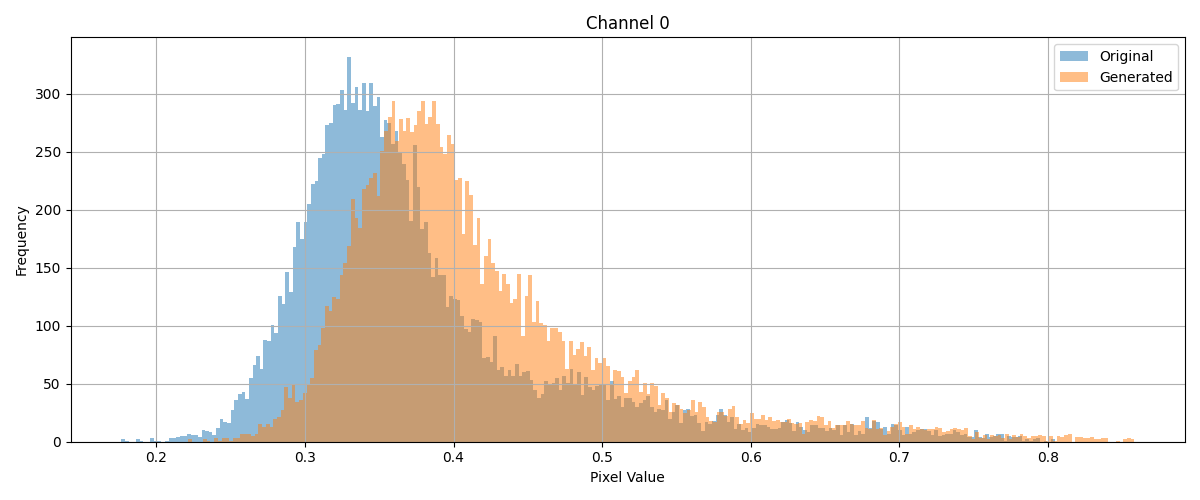
\includegraphics[width=0.9\textwidth]{images/training/cyclegan/compare_distribution_40}
        \caption{CycleGAN intensity distribution (Epoch 40).}
    \end{subfigure}
    
    \vspace{0.5cm}
    
    % Pix2Pix Distribution
    \begin{subfigure}{\textwidth}
        \centering
        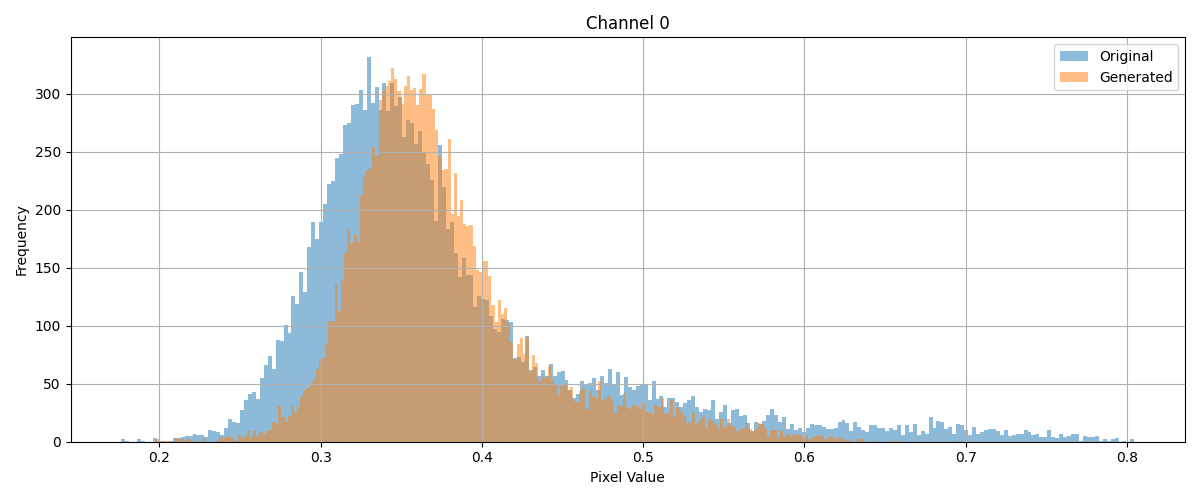
\includegraphics[width=0.9\textwidth]{images/training/pix2pix/compare_distribution_60}
        \caption{Pix2Pix intensity distribution (Epoch 60).}
    \end{subfigure}
    \caption{Comparison of pixel intensity distributions between real SHARAD observations and synthetic outputs.}
    \label{fig:app_distributions}
\end{figure}

\clearpage

% --- FIGURA 2: RANGELINES ---
\begin{figure}[htbp]
    \centering
    % CycleGAN Rangelines
    \begin{subfigure}{\textwidth}
        \centering
        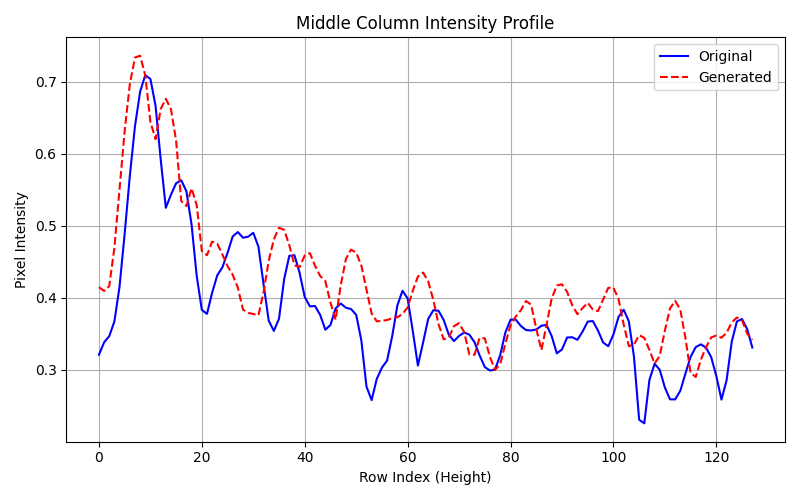
\includegraphics[width=0.9\textwidth]{images/training/cyclegan/compare_rangeline_40}
        \caption{CycleGAN average vertical rangeline (Epoch 40).}
    \end{subfigure}
    
    \vspace{0.5cm}
    
    % Pix2Pix Rangelines
    \begin{subfigure}{\textwidth}
        \centering
        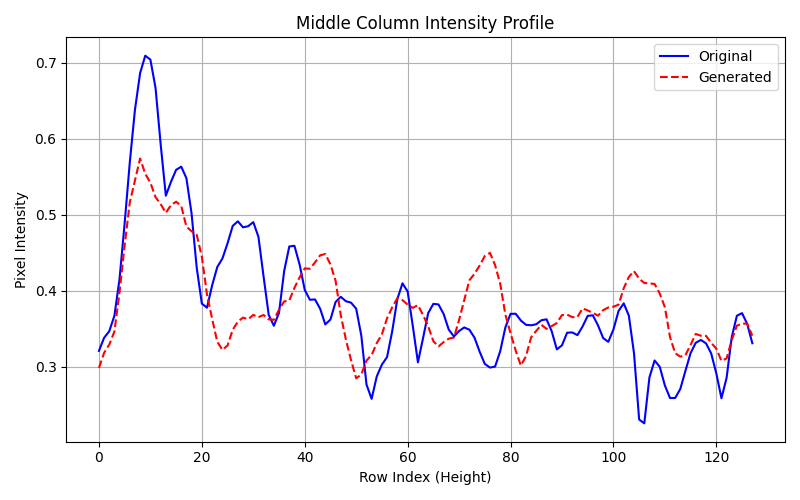
\includegraphics[width=0.9\textwidth]{images/training/pix2pix/compare_rangeline_60}
        \caption{Pix2Pix average vertical rangeline (Epoch 60).}
    \end{subfigure}
    \caption{Comparison of average vertical rangelines between real SHARAD observations and synthetic outputs.}
    \label{fig:app_rangelines}
\end{figure}

\clearpage

\section{Generation Evolution Across Epochs}
The following figures present the qualitative evolution of the generator networks during training.
Each pair compares the output of Pix2Pix (left) and CycleGAN (right) at equivalent training stages, demonstrating how the networks progressively learn to synthesize realistic subsurface textures and speckle noise. \textbf{Note:} The total number of training epochs differs between the two architectures due to training configuration choices.
Consequently, the ``Final Epoch'' shown in the comparisons corresponds to Epoch 60 for Pix2Pix and Epoch 40 for CycleGAN.


\vspace{0.5cm}


% --- PAGINA 1: EPOCA 10 ---
\begin{figure}[htbp]
    \centering
    \textbf{Epoch 10} \\ \vspace{0.3cm}
    \begin{minipage}{0.48\textwidth}
        \centering
        
\includegraphics[width=\textwidth]{images/training/pix2pix/comparison_epoch_10}
        \caption*{Pix2Pix}
    \end{minipage}\hfill
    \begin{minipage}{0.48\textwidth}
        \centering
        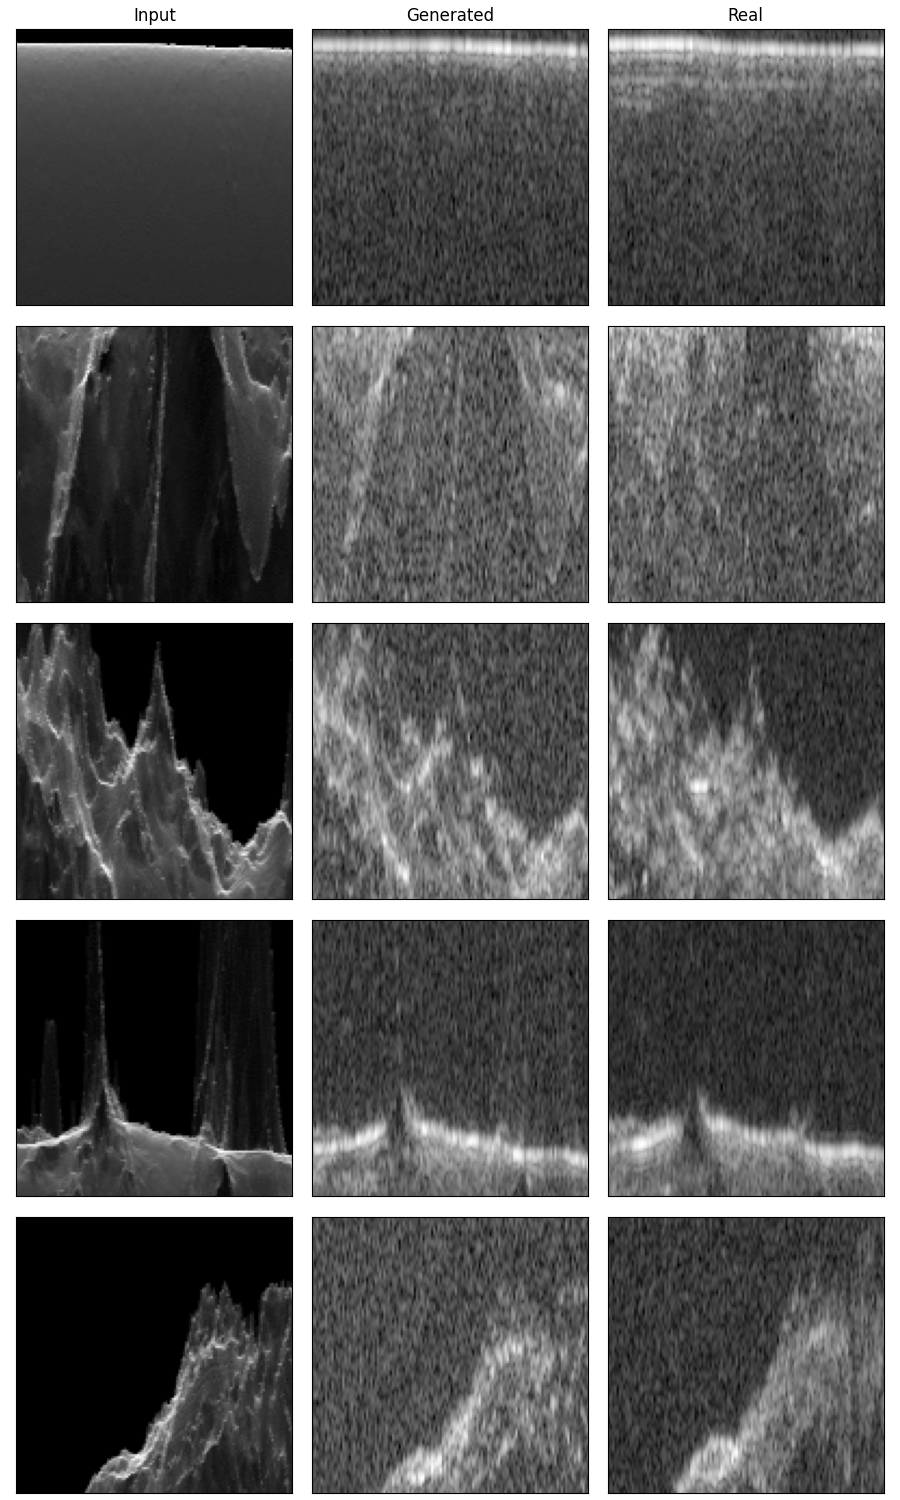
\includegraphics[width=\textwidth]{images/training/cyclegan/comparison_epoch_10}
        \caption*{CycleGAN}
    \end{minipage}
    \vspace{0.3cm}
    \caption{Qualitative generation evolution during training. (Part 1: Epoch 10)}
    \label{fig:app_evo}
\end{figure}

\clearpage

% --- PAGINA 2: EPOCA 20 ---
\begin{figure}[htbp]
    \ContinuedFloat
    \centering
    \textbf{Epoch 20} \\ \vspace{0.3cm}
    \begin{minipage}{0.48\textwidth}
        \centering
        
\includegraphics[width=\textwidth]{images/training/pix2pix/comparison_epoch_20}
        \caption*{Pix2Pix}
    \end{minipage}\hfill
    \begin{minipage}{0.48\textwidth}
        \centering
        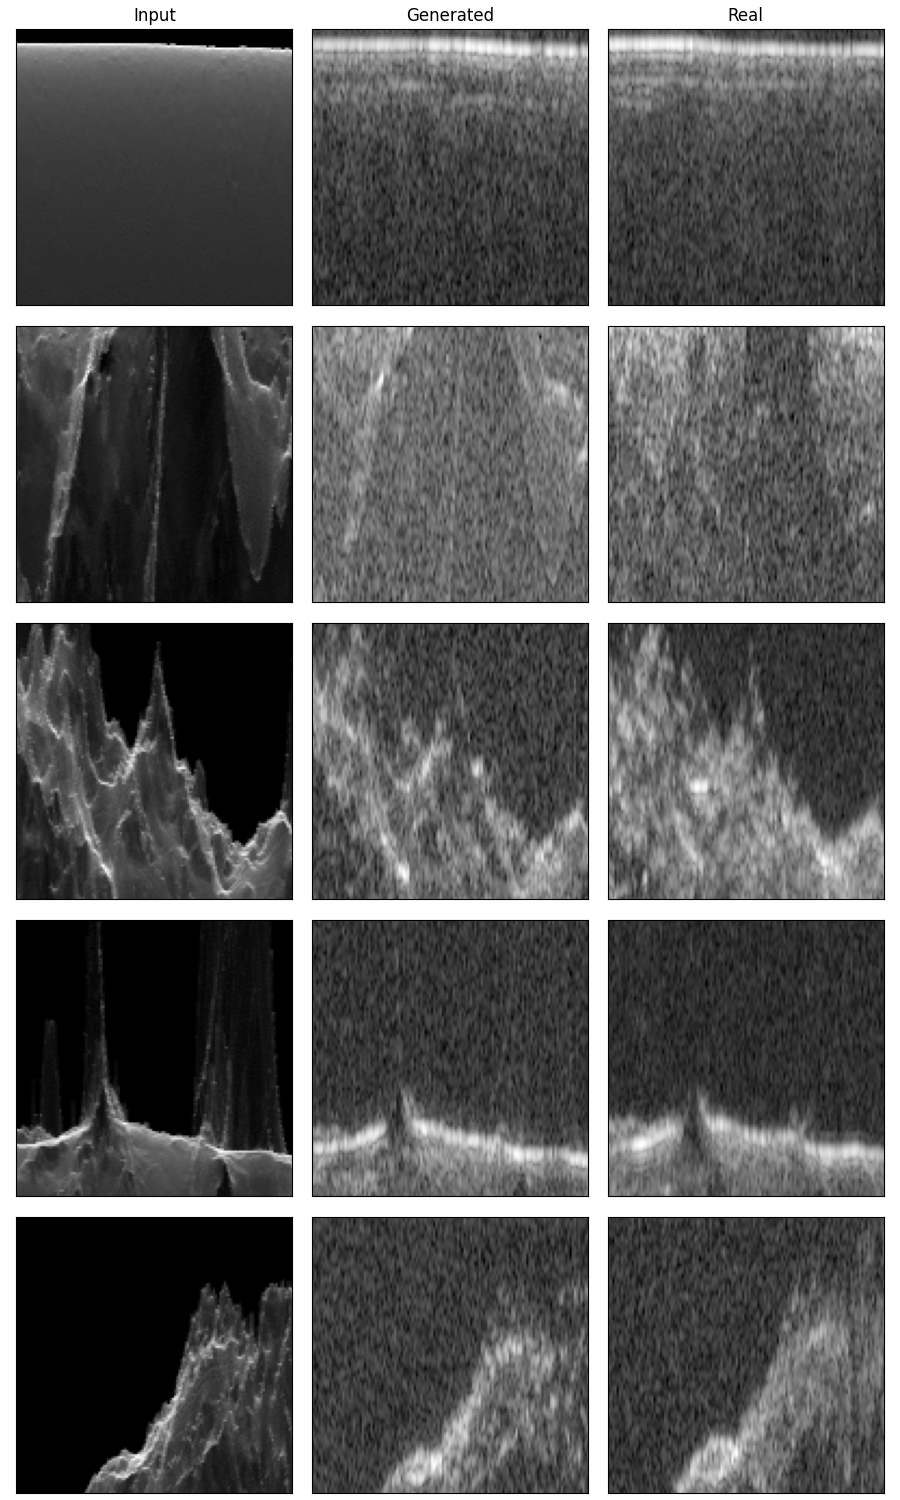
\includegraphics[width=\textwidth]{images/training/cyclegan/comparison_epoch_20}
        \caption*{CycleGAN}
    \end{minipage}
    \vspace{0.3cm}
    \caption{Qualitative generation evolution during training. (Part 2: Epoch 20)}
\end{figure}

\clearpage

% --- PAGINA 3: EPOCA 30 ---
\begin{figure}[htbp]
    \ContinuedFloat
    \centering
    \textbf{Epoch 30} \\ \vspace{0.3cm}
    \begin{minipage}{0.48\textwidth}
        \centering
        
\includegraphics[width=\textwidth]{images/training/pix2pix/comparison_epoch_30}
        \caption*{Pix2Pix}
    \end{minipage}\hfill
    \begin{minipage}{0.48\textwidth}
        \centering
        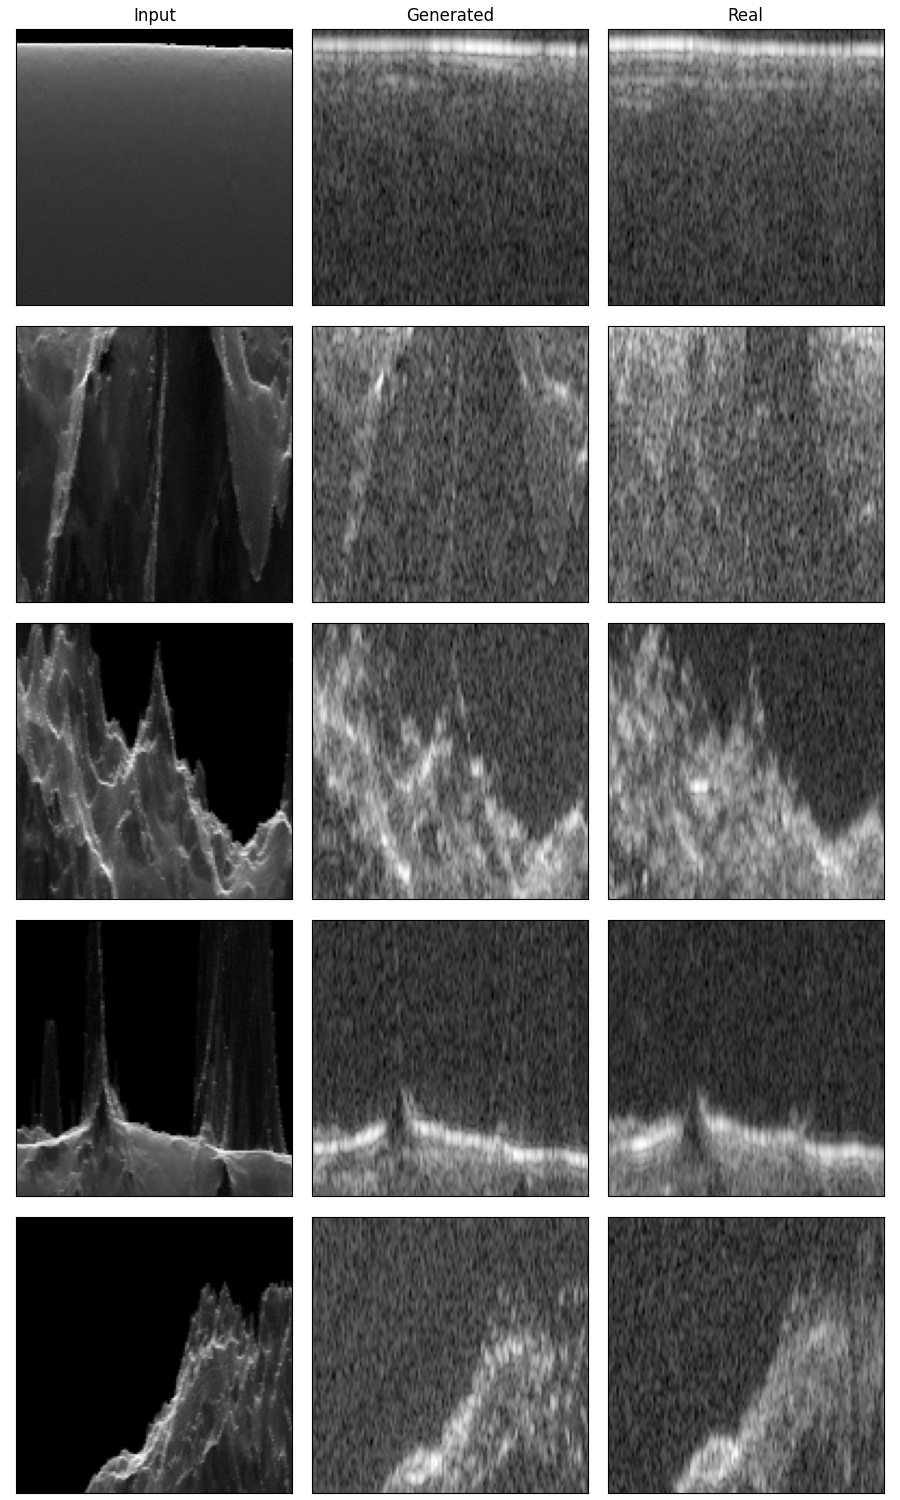
\includegraphics[width=\textwidth]{images/training/cyclegan/comparison_epoch_30}
        \caption*{CycleGAN}
    \end{minipage}
    \vspace{0.3cm}
    \caption{Qualitative generation evolution during training. (Part 3: Epoch 30)}
\end{figure}

\clearpage

% --- PAGINA 4: EPOCA FINALE ---
\begin{figure}[htbp]
    \ContinuedFloat
    \centering
    \textbf{Final Epoch} \\ \vspace{0.3cm}
    \begin{minipage}{0.48\textwidth}
        \centering
        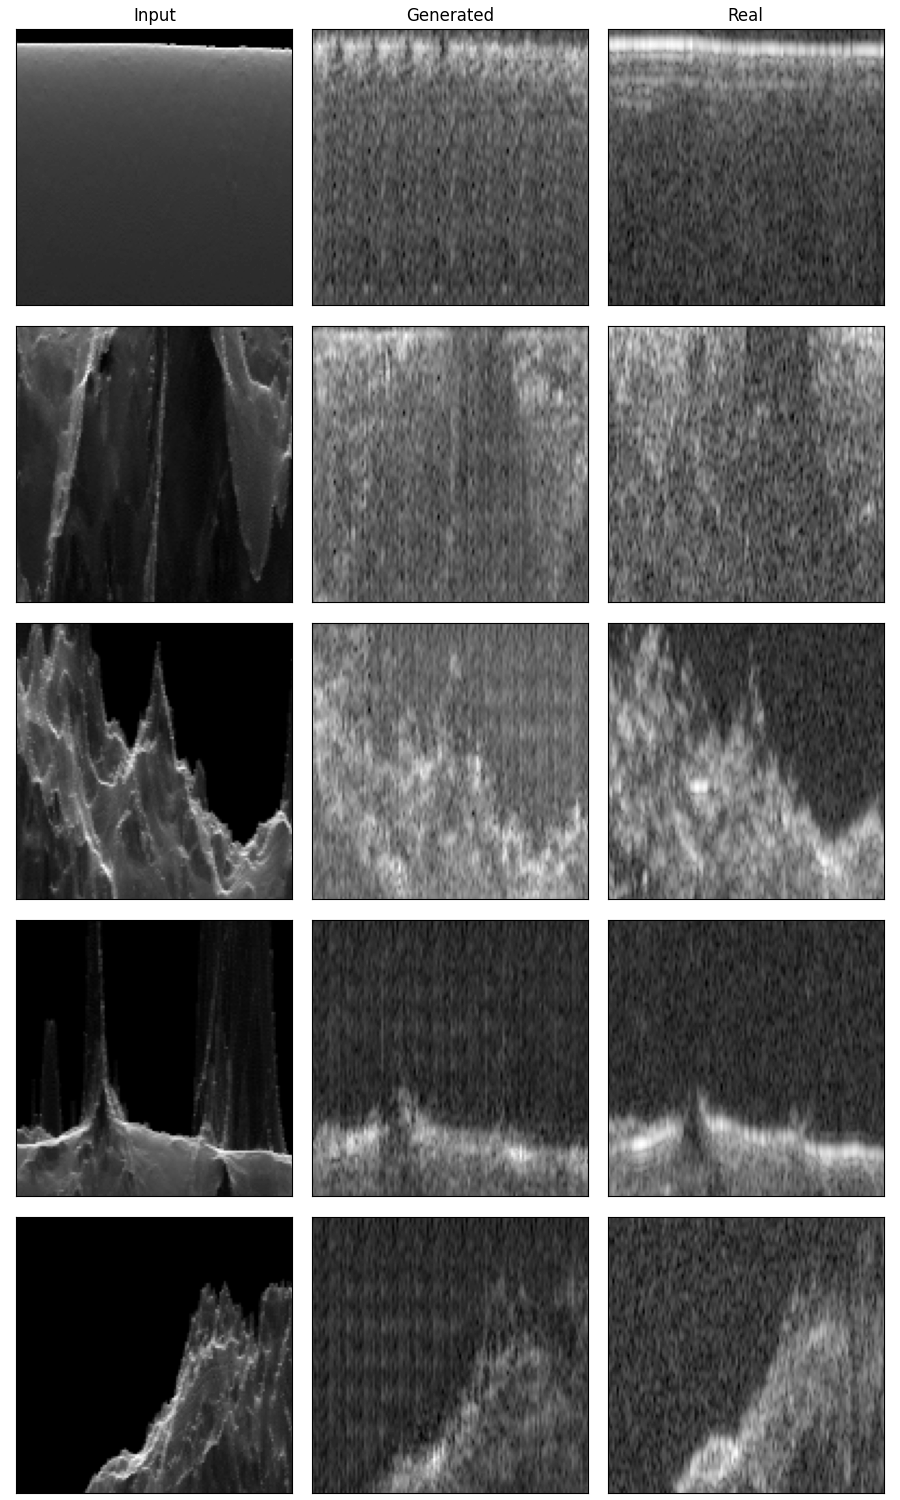
\includegraphics[width=\textwidth]{images/training/pix2pix/comparison_epoch_60}
        \caption*{Pix2Pix (Epoch 60)}
    \end{minipage}\hfill
    \begin{minipage}{0.48\textwidth}
        \centering
        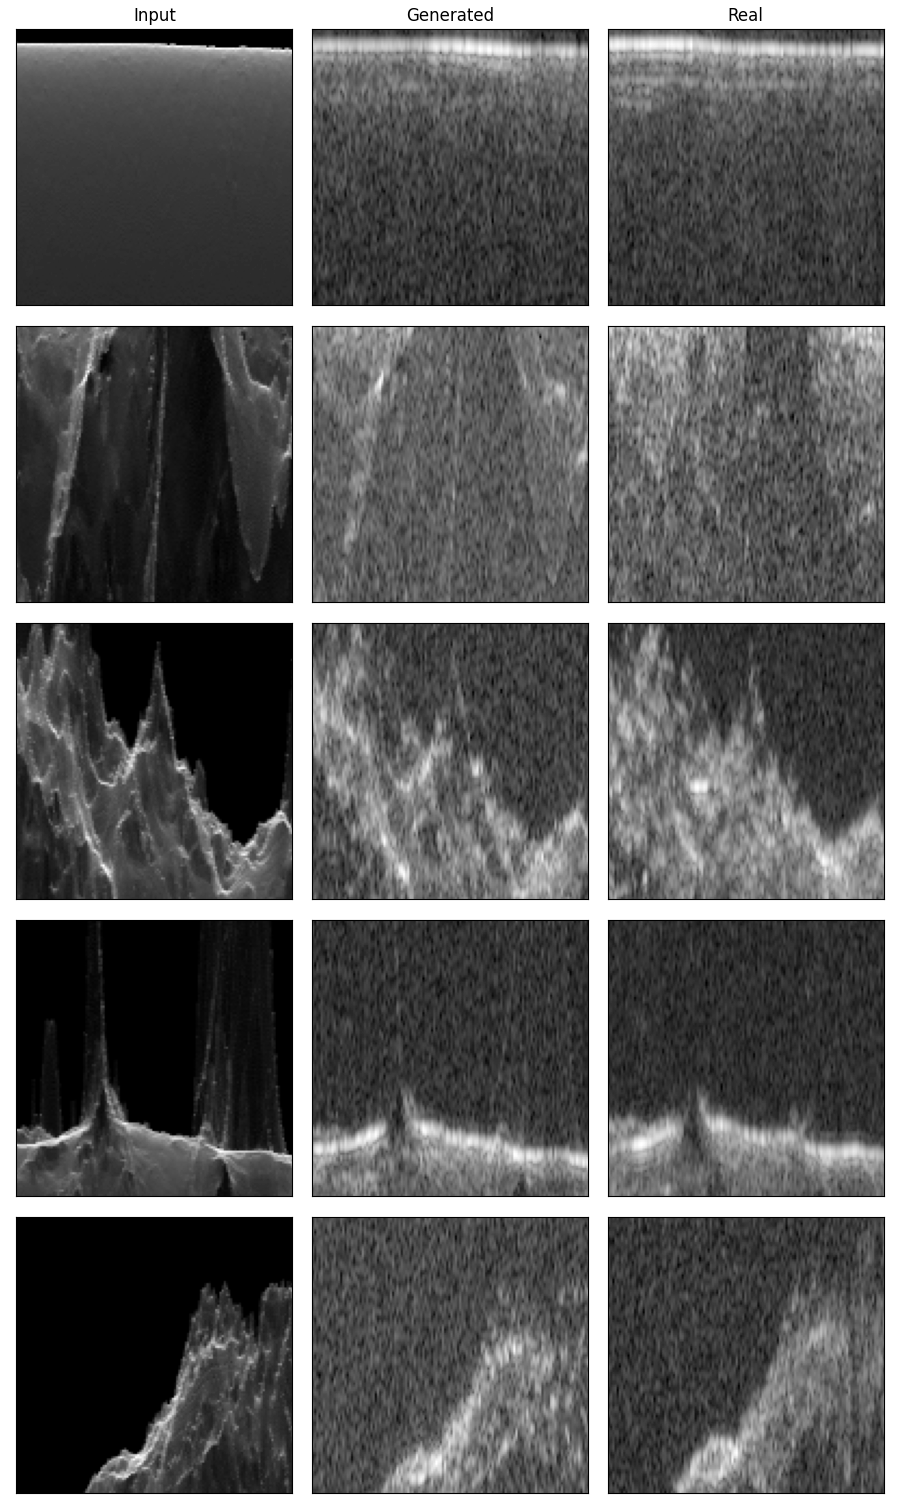
\includegraphics[width=\textwidth]{images/training/cyclegan/comparison_epoch_40}
        \caption*{CycleGAN (Epoch 40)}
    \end{minipage}
    \vspace{0.3cm}
    \caption{Qualitative generation evolution during training. (Part 4: Final Epochs)}
\end{figure}

\clearpage

